En esta sección se presentan los resultados experimentales obtenidos al medir el tiempo de ejecución y el uso de memoria de las implementaciones de los algoritmos de fuerza bruta y programación dinámica para la detección de diferencias entre dos secuencias. Los datos fueron generados utilizando scripts en Python que ejecutan los programas sobre archivos de entrada generados previamente con distintos tamaños de entrada $k$ (número de casos). Todos los archivos generados se encuentran disponibles en la carpeta \texttt{data}.

\subsection{Metodología de experimentación}

Se generaron múltiples archivos de entrada con un número de casos creciente, desde $k=10$ hasta $k=10^7$, usando secuencias aleatorias de caracteres alfabéticos en mayúscula. Las longitudes de las secuencias se limitaron a 20 caracteres para la fuerza bruta y a 100 caracteres para la programación dinámica, para asegurar una ejecución razonable en ambos algoritmos.

Para la generación de los distintos inputs es necesario ejecutar para ambos algoritmos el programa \texttt{input\_generator.py} que se encuentra en la carpeta \texttt{scripts} de cada algoritmo, despues solo se requiere ejecutar el programa principal de cada algoritmo haciendo uso del comando \lstinline|make run|. 

La ejecución de cada algoritmo fue cronometrada utilizando la biblioteca \texttt{time} y el consumo de memoria fue medido con \texttt{psutil}. Posteriormente, los datos se almacenaron en archivos CSV, y las visualizaciones fueron realizadas con \texttt{matplotlib}, generando gráficos de tiempo y memoria en función de $k$, utilizando una escala logarítmica para una mejor visualización.

\subsection{Análisis de resultados}

La Figura~\ref{fig:bf-tiempo} muestra el tiempo de ejecución del algoritmo de fuerza bruta. Se observa un crecimiento exponencial, pero para efectos prácticos para valores $k$ mayores a $1.000$ se puso como valor por defecto un tiempo de 60 segundos, esto puesto que para valores de $k$ mayores a $1.000$, el tiempo de ejecución se volvia demasiado extenso, lo cual confirma su ineficiencia frente a grandes volúmenes de datos.

\begin{figure}[H]
    \centering
    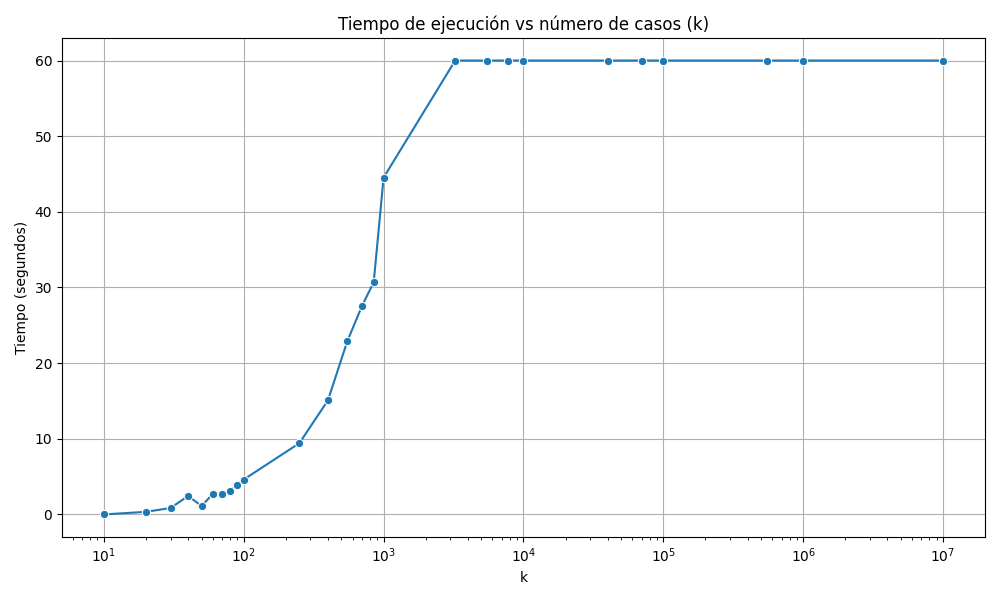
\includegraphics[width=0.8\textwidth]{../code/brute_force/data/plots/tiempo_vs_k.png}
    \caption{Tiempo de ejecución vs número de casos $k$ para algoritmo de fuerza bruta.}
    \label{fig:bf-tiempo}
\end{figure}

En la Figura~\ref{fig:bf-memoria}, que representa el uso de memoria del algoritmo de fuerza bruta, se observan valores anómalos extremadamente altos (del orden de $10^{19}$ MB), debido a que se fijo tambien el valor de la memoria con $k$ mayor a $1.000$. Sin embargo, en general, el consumo de memoria no escala significativamente con $k$, dado que cada subproblema es procesado de forma independiente y no se almacenan estructuras auxiliares significativas.

\begin{figure}[H]
    \centering
    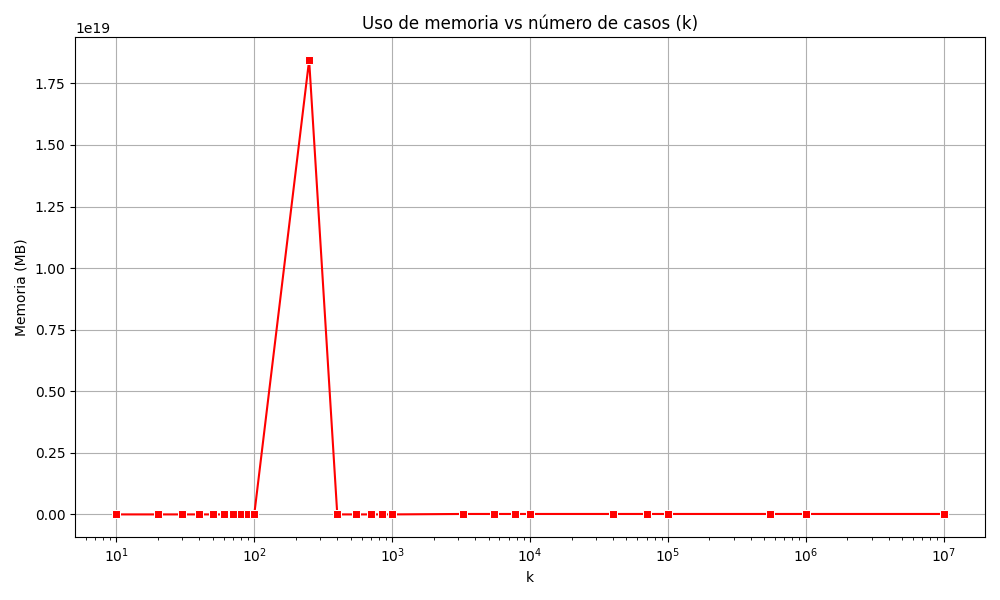
\includegraphics[width=0.8\textwidth]{../code/brute_force/data/plots/memoria_vs_k.png}
    \caption{Uso de memoria vs número de casos $k$ para algoritmo de fuerza bruta.}
    \label{fig:bf-memoria}
\end{figure}

Por otro lado, la Figura~\ref{fig:dp-tiempo} muestra el tiempo de ejecución del algoritmo de programación dinámica. En este caso, el algoritmo muestra un crecimiento mucho más controlado del tiempo de ejecución, manteniéndose por debajo de los 8 segundos incluso para $k = 10^7$. Esto es consistente con la complejidad $O(nm)$ de este enfoque, que resulta mucho más eficiente al aumentar la cantidad de casos.

\begin{figure}[H]
    \centering
    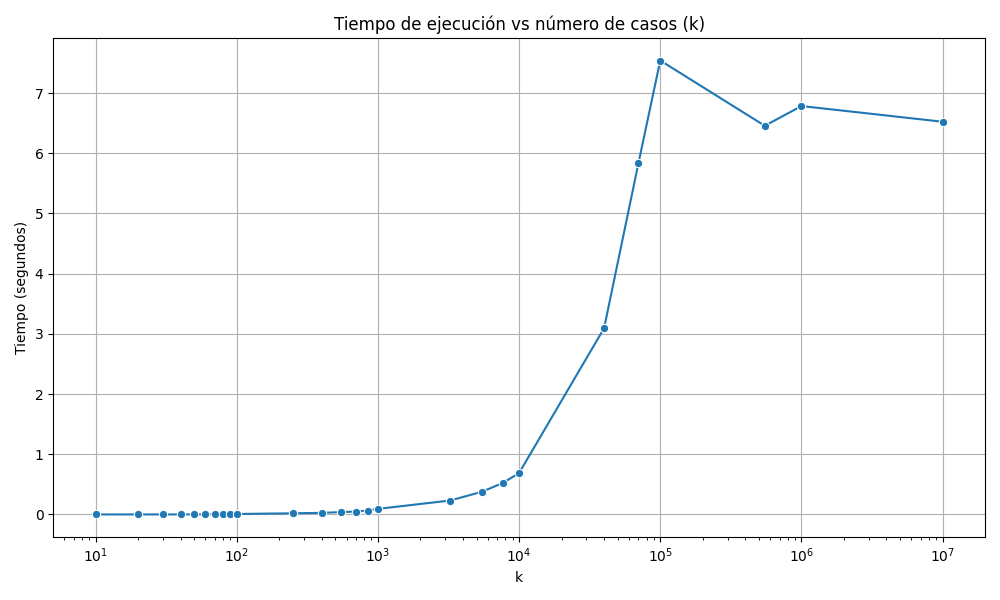
\includegraphics[width=0.8\textwidth]{../code/dynamic_programming/data/plots/tiempo_vs_k.png.png}
    \caption{Tiempo de ejecución vs número de casos $k$ para algoritmo de programación dinámica.}
    \label{fig:dp-tiempo}
\end{figure}

La Figura~\ref{fig:dp-memoria} muestra el uso de memoria del algoritmo de programación dinámica. Al igual que con el enfoque de fuerza bruta, se presentan algunos picos anómalos en los valores medidos. Estos valores no son consistentes con el comportamiento real del algoritmo, que debería tener un uso de memoria lineal respecto al número de casos y cuadrático respecto a la longitud máxima de las secuencias.

\begin{figure}[H]
    \centering
    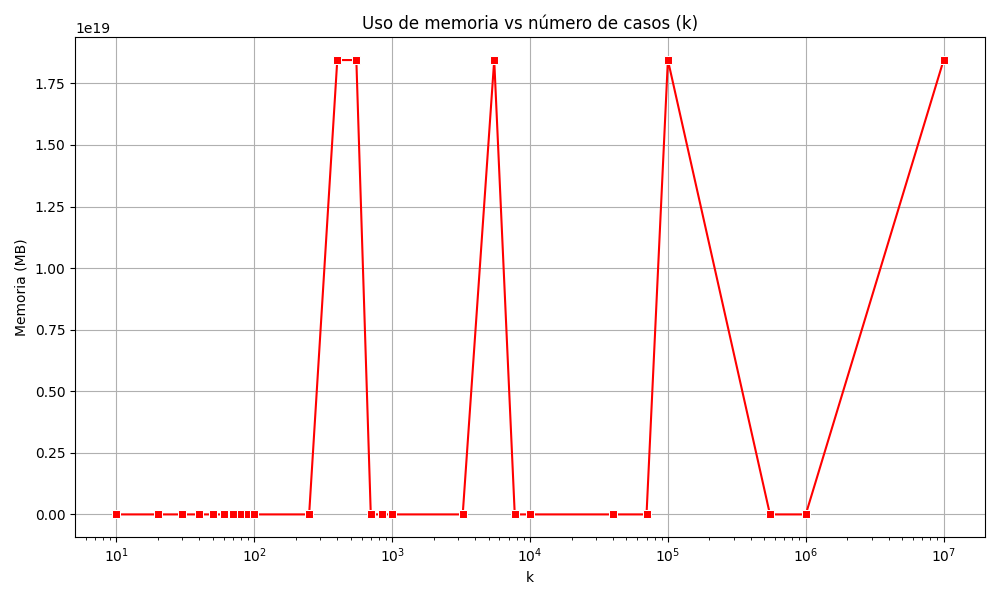
\includegraphics[width=0.8\textwidth]{../code/dynamic_programming/data/plots/memoria_vs_k.png}
    \caption{Uso de memoria vs número de casos $k$ para algoritmo de programación dinámica.}
    \label{fig:dp-memoria}
\end{figure}